\documentclass[a4paper]{article}
\usepackage[utf8x]{inputenc}
\usepackage[T1,T2A]{fontenc}
\usepackage[russian]{babel}
\usepackage{hyperref}
\usepackage{indentfirst}
\usepackage{listings}
\usepackage{color}
\usepackage{here}
\usepackage{array}
\usepackage{multirow}
\usepackage{graphicx}
\setcounter{tocdepth}{3}

\usepackage{caption}
\renewcommand{\lstlistingname}{Программа} % заголовок листингов кода

\usepackage{listings}
\lstset{ %
extendedchars=\true,
keepspaces=true,
language=bash,					% choose the language of the code
basicstyle=\footnotesize,		% the size of the fonts that are used for the code
numbers=left,					% where to put the line-numbers
numberstyle=\footnotesize,		% the size of the fonts that are used for the line-numbers
stepnumber=1,					% the step between two line-numbers. If it is 1 each line will be numbered
numbersep=5pt,					% how far the line-numbers are from the code
backgroundcolor=\color{white},	% choose the background color. You must add \usepackage{color}
showspaces=false				% show spaces adding particular underscores
showstringspaces=false,			% underline spaces within strings
showtabs=false,					% show tabs within strings adding particular underscores
frame=single,           		% adds a frame around the code
tabsize=2,						% sets default tabsize to 2 spaces
captionpos=b,					% sets the caption-position to bottom
breaklines=true,				% sets automatic line breaking
breakatwhitespace=false,		% sets if automatic breaks should only happen at whitespace
escapeinside={\%*}{*)},			% if you want to add a comment within your code
postbreak=\raisebox{0ex}[0ex][0ex]{\ensuremath{\color{red}\hookrightarrow\space}}
}

\usepackage[left=2cm,right=2cm,
top=2cm,bottom=2cm,bindingoffset=0cm]{geometry}


\begin{document}	% начало документа

\begin{titlepage}	% начало титульной страницы

	\begin{center}		% выравнивание по центру

		\large Санкт-Петербургский Политехнический Университет Петра Великого\\
		\large Институт компьютерных наук и технологий \\
		\large Кафедра компьютерных систем и программных технологий\\[6cm]
		% название института, затем отступ 6см
		
		\huge Программирование\\[0.5cm] % название работы, затем отступ 0,5см
		\large Отчет по курсовой работе\\[0.1cm]
		\large 2D-игра жанра Платформер\\[5cm]
	\end{center}


	\begin{flushright} % выравнивание по правому краю
		\begin{minipage}{0.25\textwidth} % врезка в половину ширины текста
			\begin{flushleft} % выровнять её содержимое по левому краю

				\large\textbf{Работу выполнил:}\\
				\large Осипов А. Ю.\\
				\large {Группа:} 23501/4\\
				
				\large \textbf{Преподаватель:}\\
				\large Вылегжанина К.Д.

			\end{flushleft}
		\end{minipage}
	\end{flushright}
	
	\vfill % заполнить всё доступное ниже пространство

	\begin{center}
	\large Санкт-Петербург\\
	\large \the\year % вывести дату
	\end{center} % закончить выравнивание по центру

\thispagestyle{empty} % не нумеровать страницу
\end{titlepage} % конец титульной страницы

\vfill % заполнить всё доступное ниже пространство



% Содержание
\tableofcontents
\newpage



\section{2D-игра жанра Платформер }

\subsection{Концепция приложения}

Платформер (англ. platformer) — жанр компьютерных игр, в которых основной чертой игрового процесса является прыгание по платформам, лазанье по лестницам, собирание предметов, обычно необходимых для завершения уровня. Некоторые предметы, называемые пауэр-апами (англ. power-up), наделяют управляемого игроком персонажа особой силой, которая обычно иссякает со временем (к примеру: силовое поле, ускорение, увеличение высоты прыжков). Коллекционные предметы, оружие и «пауэер-ап» собираются обычно простым прикосновением персонажа и для применения не требуют специальных действий со стороны игрока. Реже предметы собираются в «инвентарь» героя и применяются специальной командой (такое поведение более характерно для аркадных головоломок). Сходный жанр компьютерных игр SideScroller.
Противники (называемые «врагами»), всегда многочисленные и разнородные, обладают примитивным искусственным интеллектом, стремясь максимально приблизиться к игроку, либо не обладают им вовсе, перемещаясь по круговой дистанции или совершая повторяющиеся действия. Соприкосновение с противником обычно отнимает жизненные силы у героя или вовсе убивает его. Иногда противник может быть нейтрализован либо прыжком ему на голову, либо из оружия, если им обладает герой. Смерть живых существ обычно изображается упрощённо или символически (существо исчезает или проваливается вниз за пределы экрана).
Уровни, как правило, изобилуют секретами (скрытые проходы в стенах, высокие или труднодоступные места), нахождение которых существенно облегчает прохождение и подогревает интерес игрока.
Игры подобного жанра характеризуются нереалистичностью, рисованной мультяшной графикой. Героями таких игр обычно бывают мифические существа (к примеру: драконы, гоблины) или антропоморфные животные.
Платформеры появились в начале 1980-х и стали трёхмерными ближе к концу 1990-х. Через некоторое время после образования жанра у него появилось данное название, отражающее тот факт, что в платформерах геймплей сфокусирован на прыжках по платформам в противовес стрельбе. Правда, во многих платформерах присутствует стрелковое оружие, в таких, например, как Blackthorne или Castlevania.

\subsection{Задание}

Разработать 2D игровое приложение под ОС Windows и Android. Приложение представляет собой 2D-экшн игру. Пользователю предлагается управлять двухмерным персонажем в аналогичном мире, разбитом на уровни. Для прохождения каждого уровня необходимо выполнить задание уровня, например: доставить персонажа в финальную точку уровня, уничтожить всех противников, выживать в течение некоторого времени и.т.д. Основное отличие жанра "Платформер" состоит в том, что игровой мир плоский (вид сбоку) и разбит на несколько уровней по вертикали, на каждом из которых может находиться наш песонаж.

\subsection{Минимально работоспособный продукт}

Небольшая игра, которая позволяет пользователю управлять персонажем в двухмерном мире с предусмотренной физикой и возможностью окончания игры. 

\subsection{Вывод}

Пояснён выбор темы курсового проекта. Описана концепция игрового положения "Платформер". Определено задание.

%#######################################################################################################

\section{Проектирование приложения}

\subsection{Архитектура приложения}

Приложение было разбито на 2 модуля:
\begin{enumerate}  
\item[•] core - основной набор классов для реализации игровой логики
\item[•] desktop - лаунчер для запуска приложения на ОС Windows
\end{enumerate}


Архитектура ядра выглядит следующим образом:
\begin{figure}[H]
	\begin{center}
		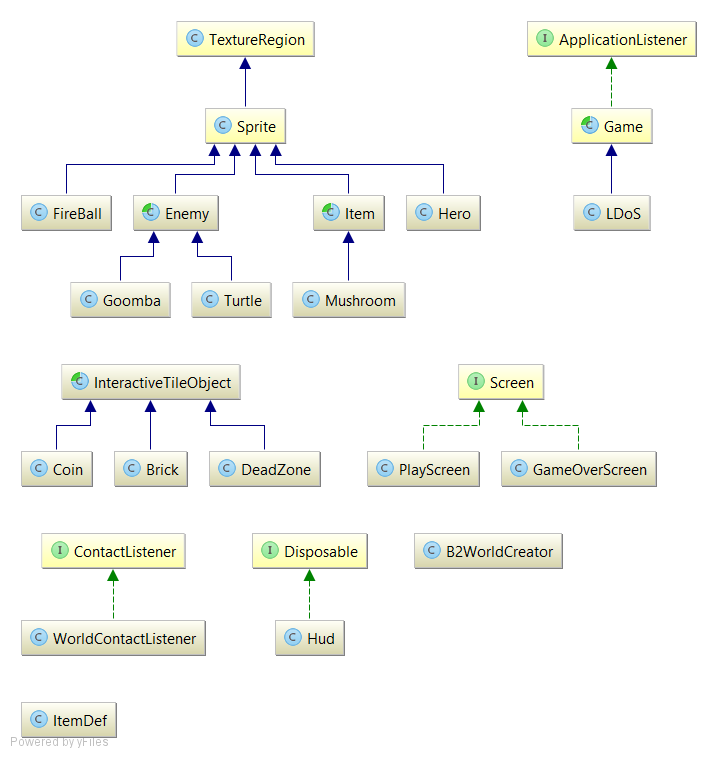
\includegraphics[scale=0.7]{pics/diagram.png}
		\caption{Диаграма классов ядра} 
		\label{pic:pic_name} % название для ссылок внутри кода
	\end{center}
\end{figure}


\subsection{Карты}

В качестве карт для приложения был выбран тип Tiled-Maps как самый простой в создании, а также обладающий широкими возможностями для редактирования. 
\\ В интернете есть большое количество Tiled-Map редакторов. Для проекта был выбран бесплатный редактор Tiled. Карты формата .tmx загружаются в проект средствами библиотеки GDX.

\section{Реализация приложения}

\subsection{Используемые версии}

\begin{enumerate}
\item[•]  IntelliJ IDEA 2016.3.1\\
Build IU-163.9166.29\\
For educational use only.\\
JRE: 1.8.0 102-b14 amd64\\
JVM: Java HotSpot(TM) 64-Bit Server VM by Oracle Corporation\\
\item[•]  Java language level: 6
\item[•]  Операционная система: Windows 10 x64
\item[•]  LibGDX 1.9.5
\item[•]  gdx-texturepacker-3.2.0
\item[•]  Tined Map Editor v3.1
\item[•]  Система автоматической сборки: Gradle 2.14
\end{enumerate}

\subsection{LibGDX и его использование при разработке игрового приложения}

LibGDX\footnote{https://libgdx.badlogicgames.com} — фреймворк для создания игр и приложений, написанный на Java с использованием C и C++ (для более быстрой работы). Он позволяет писать кроссплатформенные игры и приложения используя один код. \footnote{https://ru.wikipedia.org/wiki/LibGDX}\\

Решение, о его использование было принято по трём причинам:
\begin{enumerate}
\item[1]  Кроссплатформенность, именно благодаря этому параметру была достигнута цель создать приложение сразу под две операционные системы
\item[2]  Удобство создания графических объектов и анимации
\item[3]  Изучение нового
\end{enumerate}



\subsection{Проектирование приложения}

Классы, обеспечивающие работу приложения находятся в пакете com.mygdx.game. Для многих классов в качестве родителя был выбран класс Sprite из библиотеки LibGDX для удоства последующей отрисовки объектов этих классов. Их список приведен ниже:
\begin{enumerate}
\item[•] Hero - класс главного героя нашей игры
\item[•] Enemy - класс противника, от которого наследуются классы конкретных врагов (Turtle и Goomba)
\item[•] Item - класс для представления игровых предметов. От него наследуются следующие классы: Mushroom (на данный момент новых игровых предметов не добавлено)
\item[•] InteractiveTileObject - класс для представления интерактивных игровых объектов, т. е. объектов, с которыми может взаимодействовать игровой персонаж
\end{enumerate}

Также было создано 2 класса, обеспечивающие генерацию мира и обработку событий, которые в нем происходят:
\begin{enumerate}
\item[•] B2WorldCreator - класс, генерирующий игровой мир: на основе загруженной .tmx карты создаются игровые объекты, спавнятся противники.
\item[•] WorldContactListener - класс, использующий средства библиотеки LibGDX, обрабатывающий столкновения на основе Collision-моделей игровых объектов. 
\end{enumerate}

\subsection{Процесс создания приложения}
Процесс создания описан пошагово, затронуты ключевые пункты разработки:
\begin{enumerate}
\item[1]  Создано игровое окно
\item[2]  Создан HUD (интерфейс пользователя)
\item[3]  На основе AssetManager из LibGDX реализована подгрузка материалов
\item[4]  Создана карта с помощью Tiled Map Editor
\item[5]  Созданы спрайты игровых объектов
\item[6]  Создан персонаж и описана его основная функциональность
\item[7]  Добавлена анимация бега и прыжков
\item[8]  Реализован игровой мир на основе созданной карты, добавлено взаимодействие с интерактивными объектами
\item[9]  Добавлены звуки
\item[10]  Добавлены противники и взаимодействие с ними
\item[11]  Добавлена генерация предметов и взаимодействие с ними
\item[12]  Добавлены эффекты Power-up
\item[13]  Добавлен Game Over экран
\item[14]  Реализована смерть персонажа от противников и по истечению времени

\end{enumerate}

\subsection{Скриншоты процесса разработки}
Скриншоты процесса разработки приведены ниже:
\\
\begin{figure}[H]
	\begin{center}
		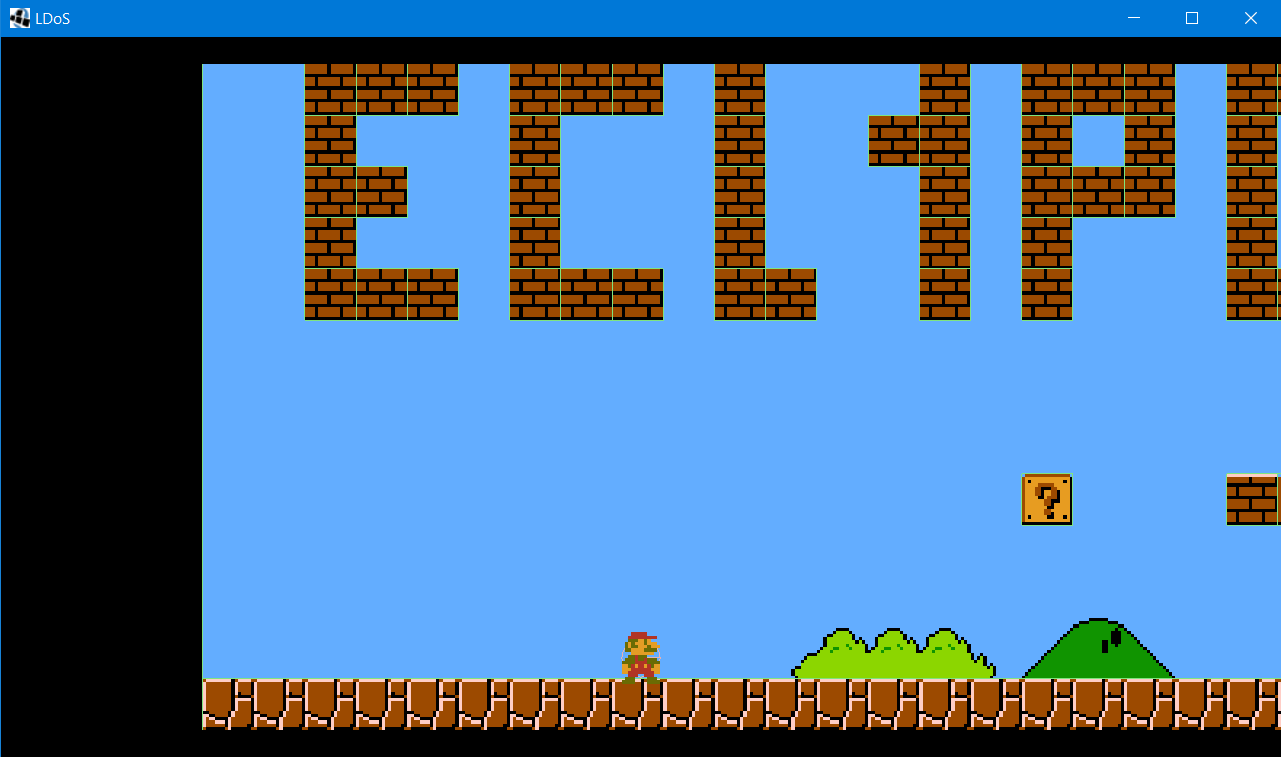
\includegraphics[scale=0.7]{pics/Screenshot_4.png}
		\caption{Игровое окно} 
		\label{pic:pic_name} % название для ссылок внутри кода
	\end{center}
\end{figure}


\begin{figure}[H]
	\begin{center}
		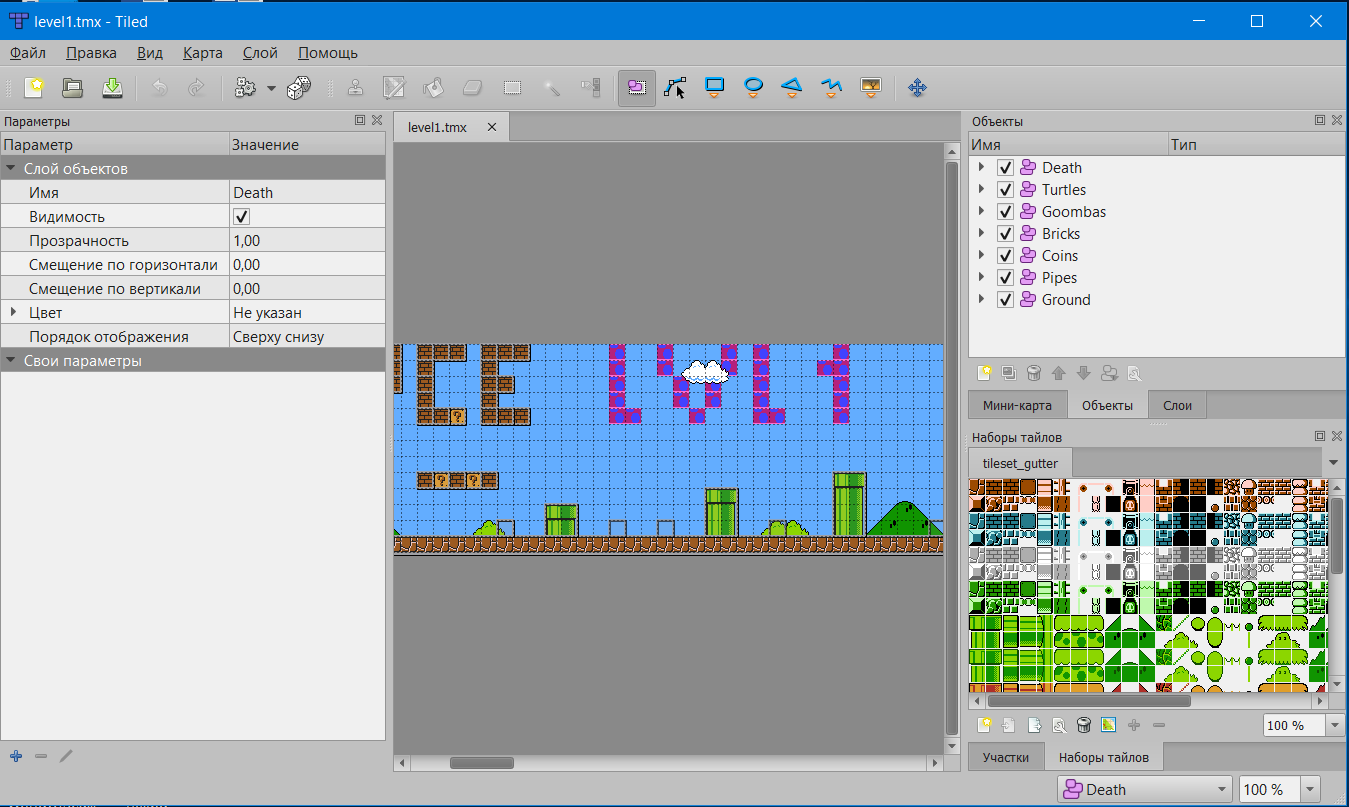
\includegraphics[scale=0.7]{pics/Screenshot_1.png}
		\caption{Разработка карты} 
		\label{pic:pic_name} % название для ссылок внутри кода
	\end{center}
\end{figure}


\begin{figure}[H]
	\begin{center}
		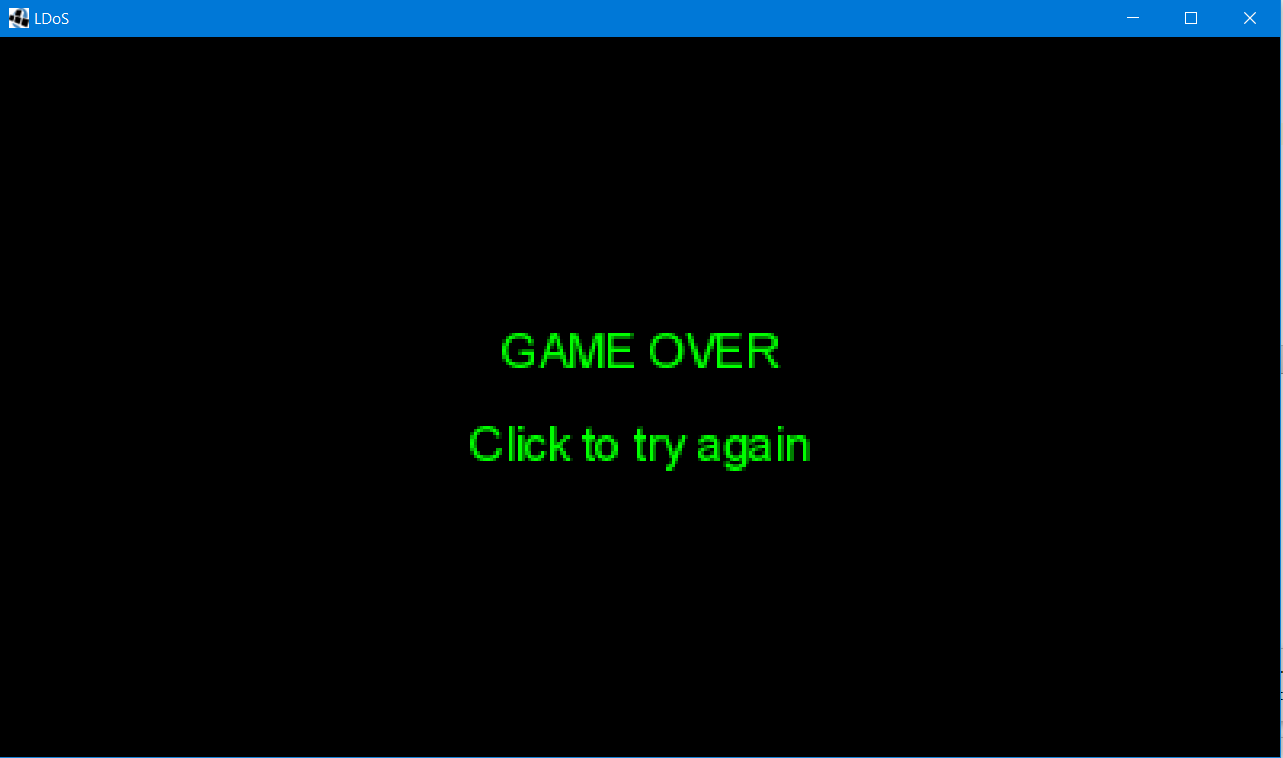
\includegraphics[scale=0.7]{pics/Screenshot_2.png}
		\caption{Game Over Screen} 
		\label{pic:pic_name} % название для ссылок внутри кода
	\end{center}
\end{figure}



\begin{figure}[H]
	\begin{center}
		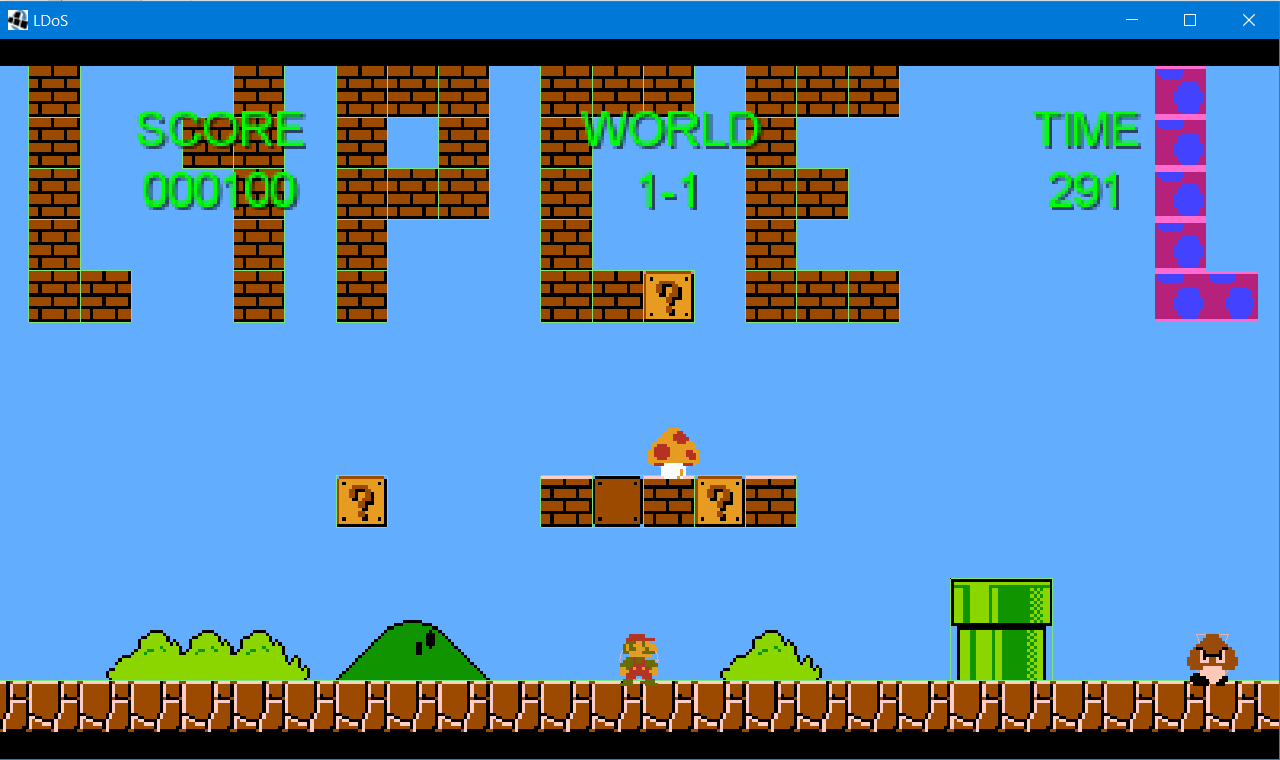
\includegraphics[scale=0.7]{pics/Screenshot_7.png}
		\caption{Mushroom} 
		\label{pic:pic_name} % название для ссылок внутри кода
	\end{center}
\end{figure}


\begin{figure}[H]
	\begin{center}
		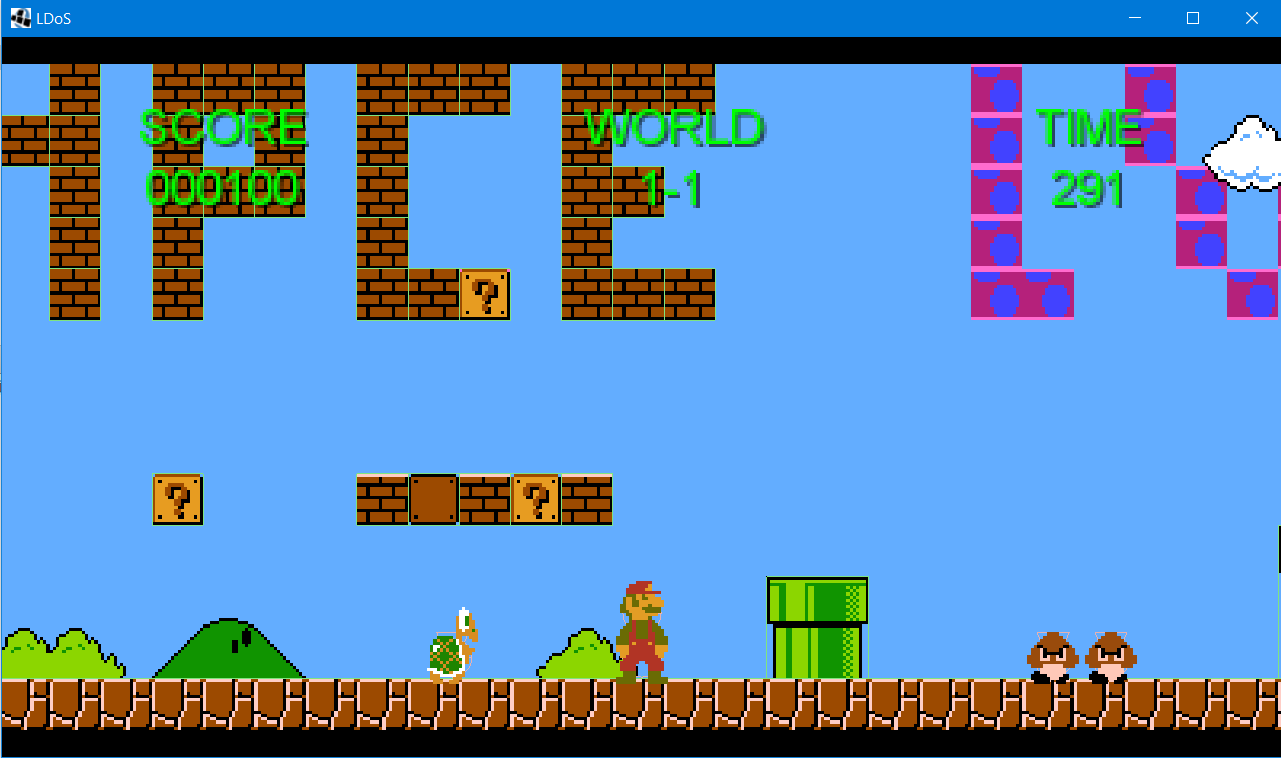
\includegraphics[scale=0.7]{pics/Screenshot_8.png}
		\caption{Противники} 
		\label{pic:pic_name} % название для ссылок внутри кода
	\end{center}
\end{figure}
 
\begin{figure}[H]
	\begin{center}
		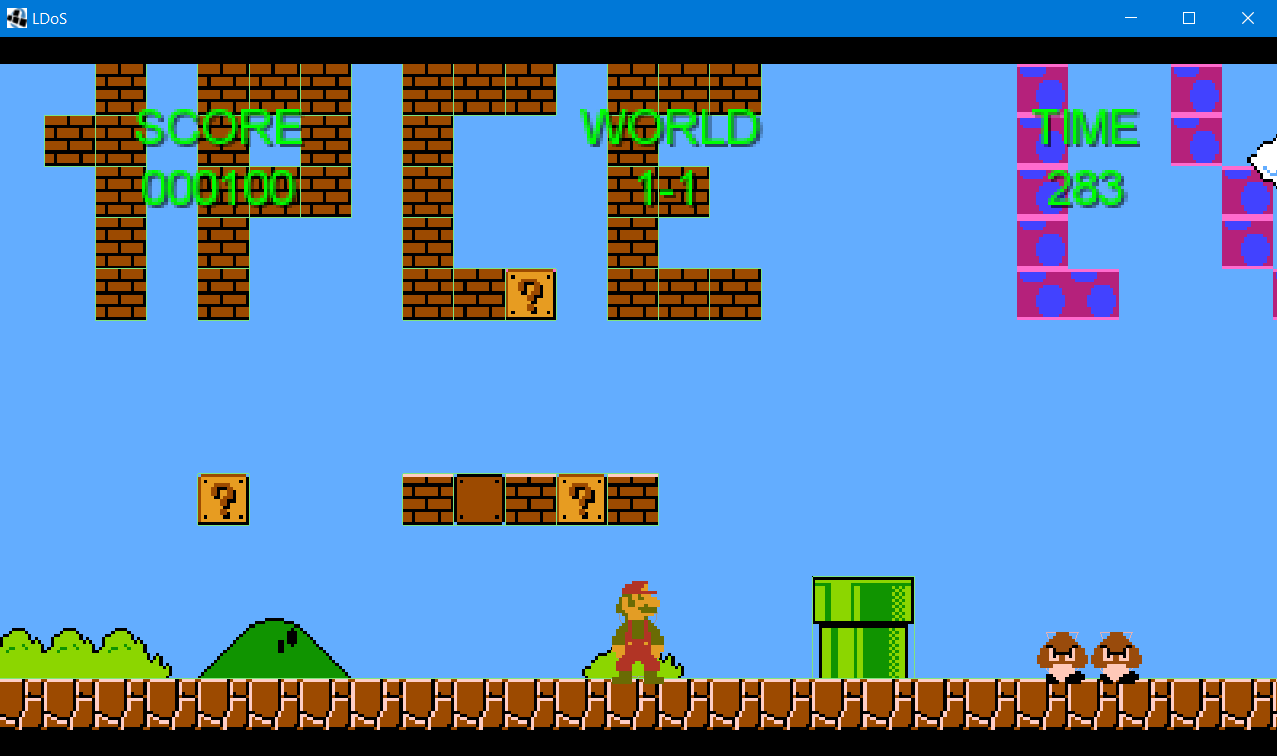
\includegraphics[scale=0.7]{pics/Screenshot_9.png}
		\caption{Разбивание блока (до)} 
		\label{pic:pic_name} % название для ссылок внутри кода
	\end{center}
\end{figure}

\begin{figure}[H]
	\begin{center}
		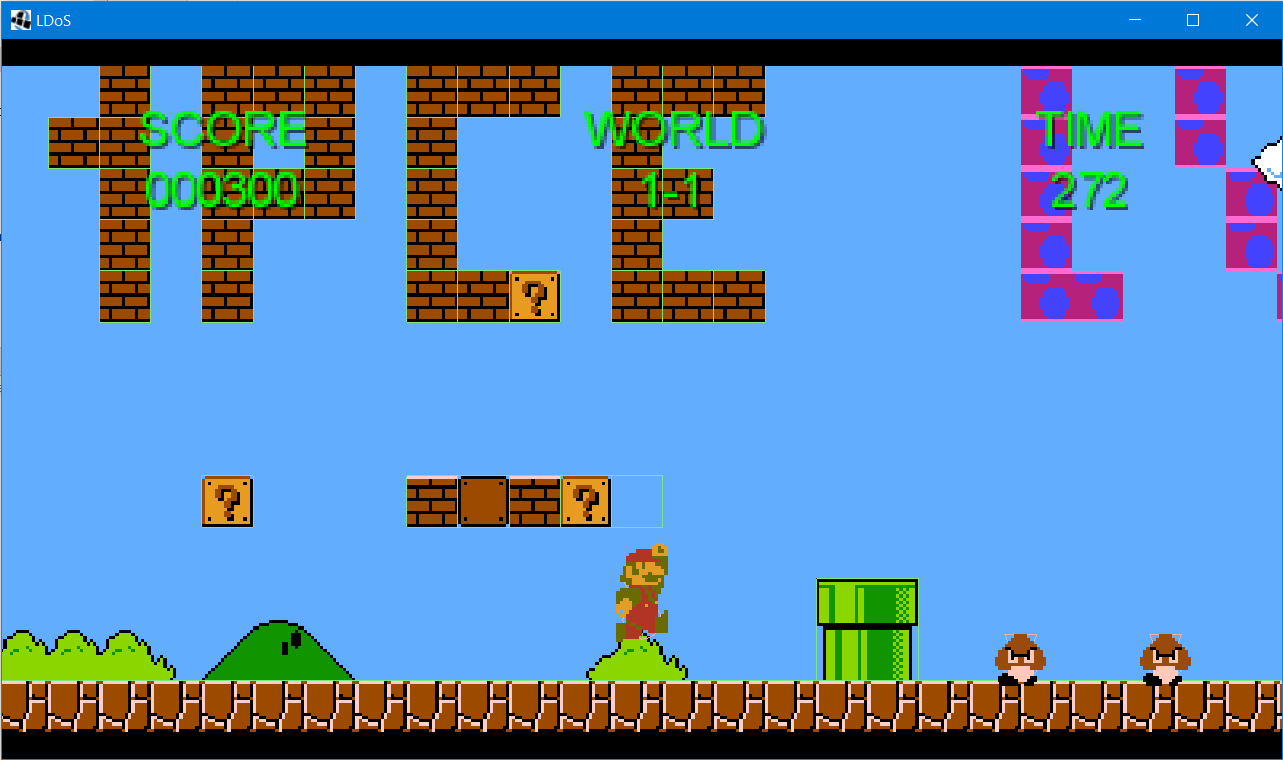
\includegraphics[scale=0.7]{pics/Screenshot_10.png}
		\caption{Разбивание блока (после)} 
		\label{pic:pic_name} % название для ссылок внутри кода
	\end{center}
\end{figure}




\subsection{Перспективы развития приложения}

Планируется реализовать следующую функциональность:
\begin{enumerate}
\item[•]  Менеджер уровней
\item[•]  Добавить сюжетную линию
\item[•]  Добавить новых противников и оружие с различной механикой
\item[•]  Добавить экран меню
\end{enumerate}

\subsection{Вывод}

Были описаны используемые средства разработки. Кратко описан фреймворк LibGDX и обосновано его использование. Был поэтапно описан процесс разработки приложения.

\section{Процесс обеспечения качества и тестирование игрового приложения Лабиринт}


Для проверки корректности работы приложения использовалось ручное тестирование.

\subsection{Тестирование}

Для ручного тестирования в приложение были добавлены логи из библиотеки LibGDX. Любое событие отображалось в консоле разработки.

Тестирование проводилось по следующему сценарию.
\begin{enumerate}
\item[•]  Запустить приложение
\item[•]  Проверить верность исполнения команд героя (прыжок, движение влево и вправо)
\item[•]  Разбить блоки
\item[•]  Различным образом взаимодействовать с врагами: прыгать на них, сталкиваться сбоку
\item[•]  Взаимодействовать с интерактивными объектами карты: брыгать на них сверху, пытаться разбить головой
\item[•]  Проверить смерть персонажа от противников и по истечению времени
\item[•]  Проверить верность отображения экрана Game Over
\item[•]  Кликнуть по нему и проверить запускание игры заново

\end{enumerate}



\subsection{Вывод}

Был описан процесс обеспечения качества и тестирования приложения.

\section{Выводы}

Было спроектирована и реализована 2D-игра жанра платформер. В процессе разработки были тточены навики програмирования на языке Java в среде InteliJ IDEA. Была изучена сторонняя библиотека LibGDX и инструмент Tiled Map Editor. В дальнейшем планируется продолжение поддержки и улучшение приложения, а также исправление текущих недочётов.

\section{Приложение}

Исходный ход можно найти в репозитории\footnote{https://github.com/Ecl1pce/LDoS} на ресурсе GitHub

\subsection{Листинги}

\lstinputlisting{../core/src/com/mygdx/game/scenes/Hud.java} 
\lstinputlisting{../core/src/com/mygdx/game/screens/GameOverScreen.java} 
\lstinputlisting{../core/src/com/mygdx/game/screens/PlayScreen.java} 
\lstinputlisting{../core/src/com/mygdx/game/sprites/enemies/Enemy.java} 
\lstinputlisting{../core/src/com/mygdx/game/sprites/enemies/Goomba.java} 
\lstinputlisting{../core/src/com/mygdx/game/sprites/enemies/Turtle.java} 
\lstinputlisting{../core/src/com/mygdx/game/sprites/items/Item.java} \lstinputlisting{../core/src/com/mygdx/game/sprites/items/ItemDef.java} 
\lstinputlisting{../core/src/com/mygdx/game/sprites/items/Mushroom.java} 
\lstinputlisting{../core/src/com/mygdx/game/sprites/other/FireBall.java} 
\lstinputlisting{../core/src/com/mygdx/game/sprites/tileObjects/Brick.java} 
\lstinputlisting{../core/src/com/mygdx/game/sprites/tileObjects/Coin.java} 
\lstinputlisting{../core/src/com/mygdx/game/sprites/tileObjects/DeadZone.java} 
\lstinputlisting{../core/src/com/mygdx/game/sprites/tileObjects/InteractiveTileObject.java} 
\lstinputlisting{../core/src/com/mygdx/game/sprites/Hero.java} 
\lstinputlisting{../core/src/com/mygdx/game/tools/B2WorldCreator.java} 
\lstinputlisting{../core/src/com/mygdx/game/tools/WorldContactListener.java} 
\lstinputlisting{../core/src/com/mygdx/game/LDoS.java} 








\end{document}
